W celu porównania trendów występujących w danych ze Stanów Zjednoczonych i Wielkiej Brytanii z danymi z Polski, przeanalizowaliśmy statystyki, które udało nam się wyciągnąć z systemu POBR \cite{pobr}.


\section{Rozkład liczby wypadków w latach}

Niestety W POBR mamy mniejszy zakres dostępnych lat niż w pozostałych bazach, pierwsze dane pochodzą z 2006 roku. Możemy jednak porównać ten okres z trendami w Wielkiej Brytanii i USA.

We wszystkich przypadkach obserwujemy spadek liczby wypadków, największa tendencja spadkowa przypada na lata 2008 - 2009, w latach 2011 - 2013 mamy do czynienia z pewnym ustabilizowaniem liczby wypadków. Można stwierdzić że trendy zaobserwowane w danych z USA i Wielkiej Brytanii znajdują potwierdzenie w danych z Polski.

\centerline{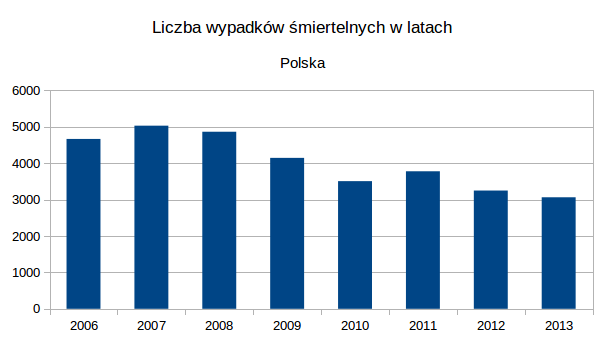
\includegraphics[width=0.9\textwidth]{images/statistics/year_pl.png}}

\centerline{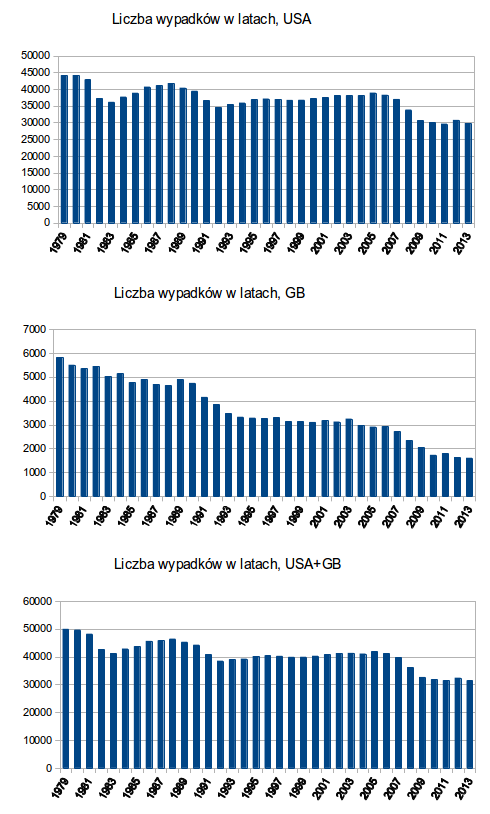
\includegraphics[width=0.9\textwidth]{images/statistics/year.png}}

\section{Liczba wypadków w zależności od typu drogi}

Wykres stworzony dla danych z Polski wykazuje duże podobieństwo do wykresu dla USA. Wykres dla Wielkiej Brytanii jest odmienny, więcej wypadków mamy dla dróg typu PRINCIPAL, bardzo mały odsetek dla dróg typu MINOR. Sugeruje to podobieństwa między siecią dróg i przyporządkowaniem ich do typów w Polsce i w Stanach Zjednoczonych.

Stały jest bardzo niski odsetek wypadków na autostradach, które są drogami mocno niekolizyjnymi. Mimo wysokich prędkości rozwijanych na takich drogach, niewielki odsetek śmiertelnych wypadków zdarza się na autostradach. Znacznie więcej śmiertelnych wypadków obserwujemy na drogach typu PRINCIPAL czyli drogach krajowych, gdzie często mamy już skrzyżowania i więcej okazji do wystąpienia kolizji. Duży procent wypadków jest też na drogach typu MINOR - czyli lokalnych, często w miastach. Mamy tam jeszcze więcej możliwości wystąpienia kolizji, więcej skrzyżowań a także więcej interakcji z pieszymi, która również może prowadzić do wypadków. \\
\\
\\


\centerline{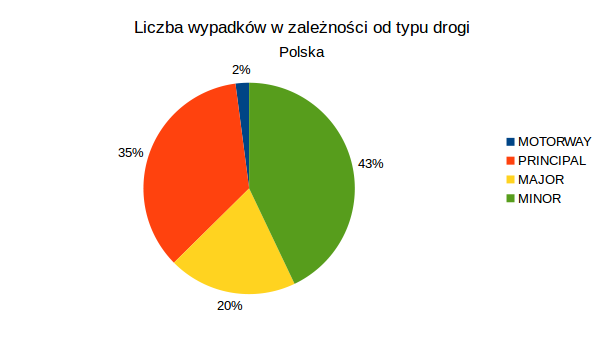
\includegraphics[width=0.9\textwidth]{images/statistics/road_type_pl.png}}

\centerline{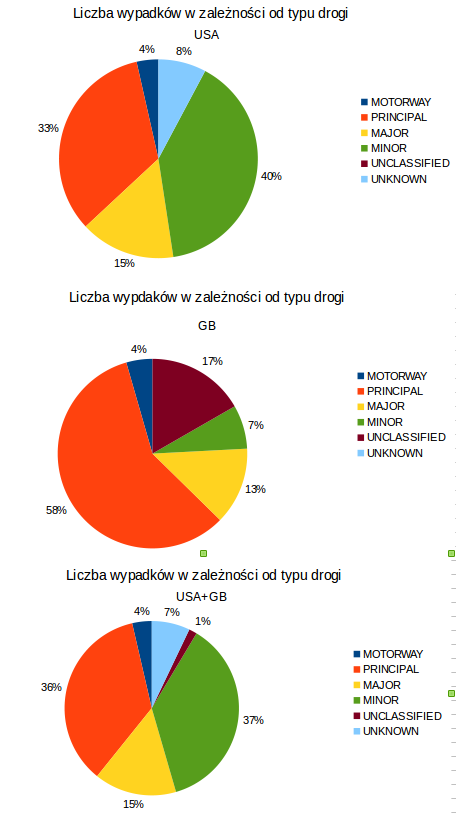
\includegraphics[width=0.8\textwidth]{images/statistics/road_type.png}}

